\documentclass[11pt]{article}
\usepackage[margin=0.75in]{geometry}
\usepackage{graphicx}
\usepackage{amsmath}
\usepackage{hyperref}
\usepackage{enumitem}
\usepackage{tikz}
\usepackage{xcolor}
\usetikzlibrary{shapes,arrows,positioning,fit,backgrounds}

\title{\textbf{Solstice: Technical Architecture}}
\author{Computer Vision + Multi-LLM Pipeline for Medical Document Verification}
\date{}

\begin{document}
\maketitle

\section{Executive Summary}

Solstice verifies medical claims against source documents using computer vision and orchestrated LLM processing. The system extracts structured content from PDFs through Detectron2, then runs claims through a four-stage LLM pipeline for evidence extraction and verification.

\section{Core Architecture}

\subsection{System Design}

Three decoupled layers handle document processing:

\begin{verbatim}
+-------------+          +---------------+          +-------------+
|   Gateway   |  <---->  | Fact Checker  |  <---->  |  Ingestion  |
+-------------+          +---------------+          +-------------+
\end{verbatim}

The Gateway accepts document uploads and claim submissions from users, returning job IDs for async processing. When a document arrives, the Ingestion layer runs first to process the PDF and extract structured JSON. Once ingestion completes, the Fact Checker can then verify claims against the cached document data using the LLM pipeline. Users poll the Gateway for results, which retrieves the evidence report once processing completes.

\subsection{Document Processing Pipeline}

\textbf{Layout Detection:}
\begin{itemize}
\item Detectron2 with ResNet-50 identifies document regions
\item 400 DPI rendering for accurate text extraction
\item Bounding box post-processing resolves overlaps
\item Outputs structured JSON with spatial coordinates
\end{itemize}

\begin{figure}[htbp]
\centering
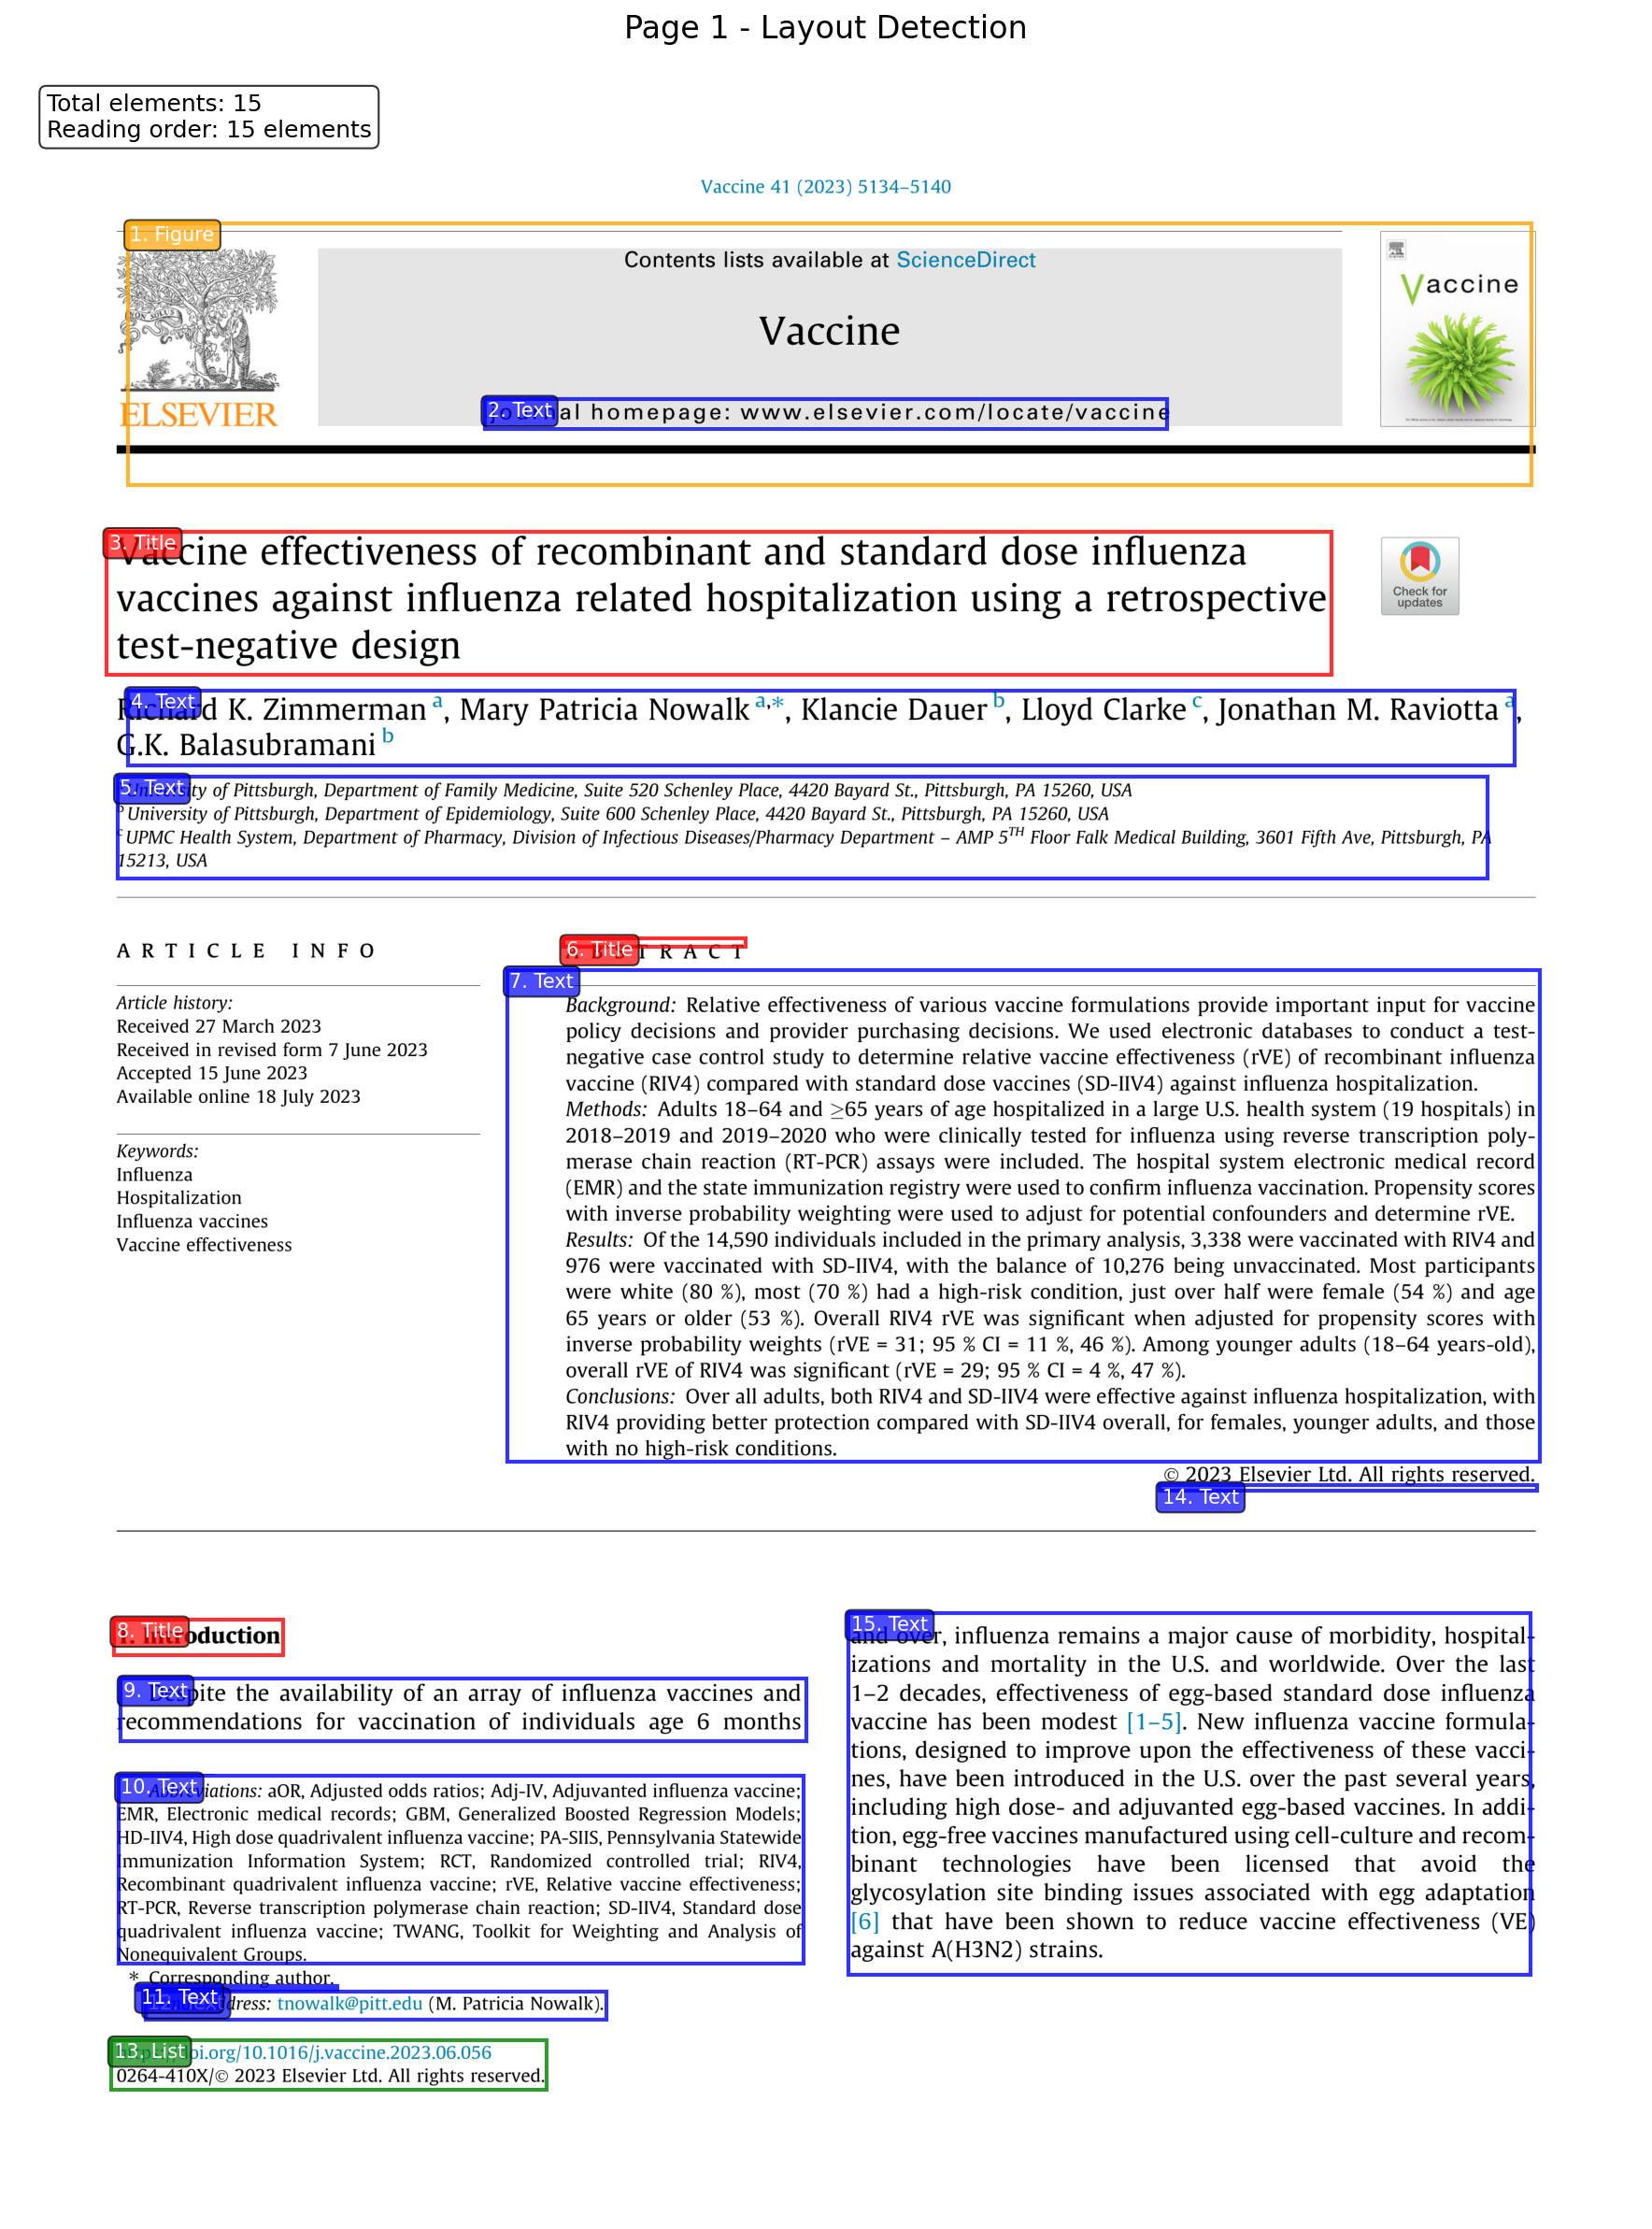
\includegraphics[width=0.85\textwidth]{scientific_layout_example.png}
\caption{Detectron2 identifies text blocks, tables, and figures in medical documents.}
\end{figure}

\section{Claim Verification Pipeline}

\subsection{Multi-Stage LLM Processing}

Claims pass through four specialized LLM components:

\newpage
\begin{verbatim}
+-----------------+     +------------------+     +-------------------+
|                 |     |                  |     |                   |
| Claim + Document|---->| Evidence        |---->| Evidence          |
|                 |     | Extractor (LLM) |     | Verifier (LLM)    |
+-----------------+     +------------------+     +---------+---------+
                                                           |
                                                           v
+-----------------+     +------------------+     +-------------------+
|                 |     |                  |     |                   |
| Images + Claim  |---->| Visual Analyzer  |     | Completeness      |
|                 |     | (Multimodal LLM) |     | Checker (LLM)     |
+-----------------+     +------------------+     +---------+---------+
                                                           |
                                                 If new evidence found
                                                           |
                                                           v
                                                 +-------------------+
                                                 | Evidence Verifier |
                                                 | (LLM) - 2nd pass  |
                                                 +-------------------+
\end{verbatim}

\subsection{LLM Components}

\textbf{Evidence Extractor}
\begin{itemize}
\item Finds quotes supporting the claim
\item Returns JSON with evidence and relevance scores
\end{itemize}

\textbf{Evidence Verifier}
\begin{itemize}
\item Validates quote accuracy against source
\item Checks for cherry-picking and missing context
\end{itemize}

\textbf{Completeness Checker}
\begin{itemize}
\item Searches for additional supporting evidence
\item Triggers second verification pass if needed
\end{itemize}

\textbf{Visual Analyzer}
\begin{itemize}
\item Processes tables/figures using multimodal LLM
\item Extracts data supporting or refuting claims
\end{itemize}

\section{Implementation Patterns}

\subsection{Orchestration}

ClaimOrchestrator manages the verification workflow:
\begin{itemize}
\item Async LLM calls with configurable timeouts
\item Exponential backoff for rate limit handling
\item State transitions through extraction, verification, and completion
\end{itemize}

\subsection{Caching Strategy}

Filesystem cache enables debugging and reprocessing:

\begin{verbatim}
data/cache/{document_name}/
    extracted/
        content.json      # Structured document content
        figures/          # Extracted images
    agents/               # LLM outputs
        claims/
            claim_{id}/
                evidence_extractor/output.json
                evidence_verifier/output.json
                completeness_checker/output.json
                image_evidence_analyzer/{figure_id}/output.json
\end{verbatim}

\section{Scaling Considerations}

\textbf{Ingestion}: CPU-bound on Detectron2, benefits from GPU acceleration

\textbf{Fact Checking}: I/O bound on LLM APIs, scales with concurrent claims

\textbf{Gateway}: Stateless handlers scale horizontally

\section{Marketing Document Adaptation}

Marketing materials use adjusted parameters:
\begin{itemize}
\item Lower confidence threshold (0.1 vs 0.2)
\item Enhanced overlap resolution for creative layouts
\item Same LLM prompts maintain consistency
\end{itemize}

\begin{figure}[htbp]
\centering
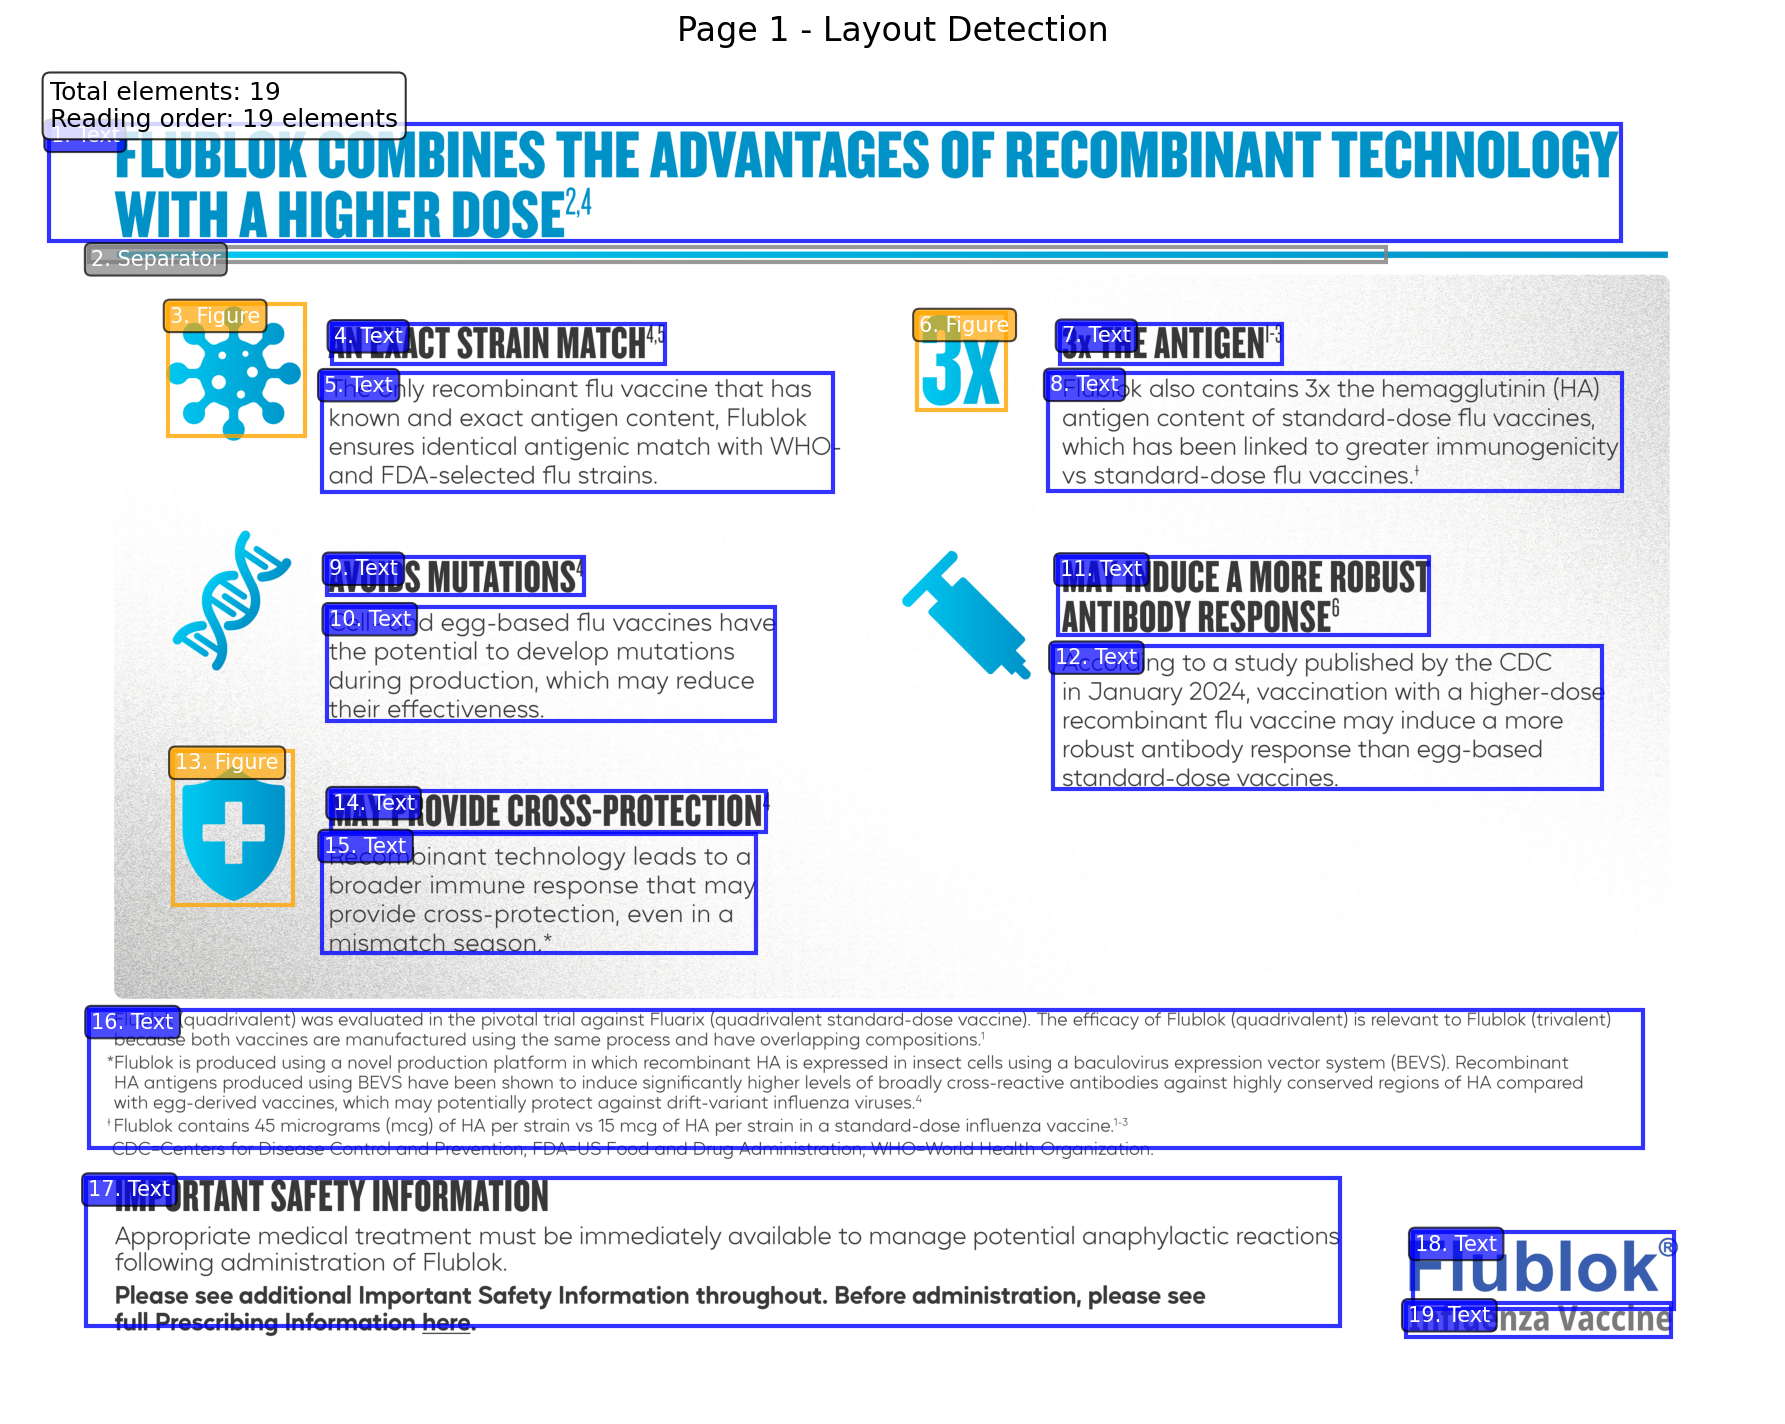
\includegraphics[width=0.85\textwidth]{marketing_layout_example.png}
\caption{Marketing documents require lower confidence thresholds for design-heavy layouts.}
\end{figure}

\end{document}